\documentclass[tikz,border=2pt]{standalone}
\usepackage{amsmath}
\usetikzlibrary{arrows.meta}
\begin{document}
% Private costs: Theta_i = {1/4, 2}, A_i = {C, D}. A pure strategy maps each type to an action,
% so there are 2^2 = 4 strategies (C,C), (C,D), (D,C), (D,D) (first entry: low-cost type).
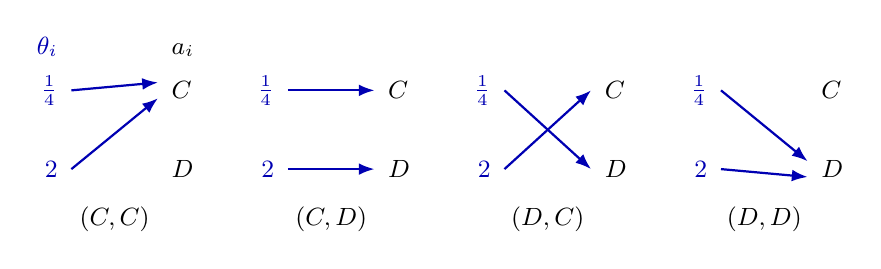
\begin{tikzpicture}[font=\small, >={Latex[length=2mm]}]
  % \a, \b: end height of the arrow from type 1/4 and from type 2
  \foreach \k/\a/\b/\name in {0/0.6/0.4/{(C,C)}, 1/0.5/-0.5/{(C,D)}, 2/-0.5/0.5/{(D,C)}, 3/-0.4/-0.6/{(D,D)}} {
    \begin{scope}[xshift=\k*2.75cm]
      \node[blue!70!black, anchor=east] at (0,0.5) {$\tfrac14$};
      \node[blue!70!black, anchor=east] at (0,-0.5) {$2$};
      \node[anchor=west] at (1.2,0.5) {$C$};
      \node[anchor=west] at (1.2,-0.5) {$D$};
      \draw[->, thick, blue!70!black] (0.05,0.5) -- (1.15,\a);
      \draw[->, thick, blue!70!black] (0.05,-0.5) -- (1.15,\b);
      \node[anchor=north] at (0.6,-0.85) {$\name$};
    \end{scope}
  }
  \node[blue!70!black, anchor=south east] at (0,0.8) {$\theta_i$};
  \node[anchor=south west] at (1.2,0.8) {$a_i$};
\end{tikzpicture}
\end{document}
